\documentclass[a4paper, 11pt]{article}


\usepackage[czech]{babel}
\usepackage[utf8]{inputenc}
\usepackage[left=2cm, top=2cm, bottom=3cm, text={17cm, 24cm}]{geometry}
\usepackage{times}
\usepackage{graphicx}
\usepackage[linesnumbered,ruled]{algorithm2e}
\usepackage{algorithmic}
\usepackage{listings}


\begin{document}


	
			\begin{center}
				{\Large
					Vysoké učení technické v~Brně \\
					Fakulta informačních technologií \\
				}
				{
\includegraphics[width=0.4\linewidth]{pic/FIT_logo.pdf}} \\

				{\LARGE
					Návrh číslicových systémů \\
					Projekt \\[0.4cm]
				}

				{\large
					Elizaveta Syanova (xsyano00) \\
					\today
				}
			\end{center}
	

    \section{Architektura navrženého obvodu (na úrovní RTL)}
	\subsection{Schéma obvodu}
	
	\begin{center}
	     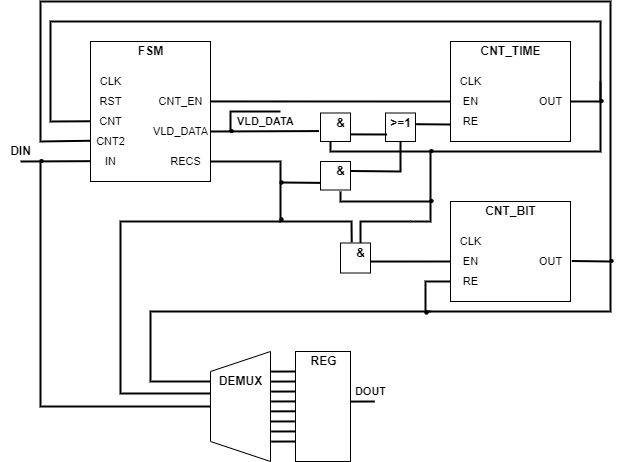
\includegraphics[width=0.85\linewidth]{pic/2ONE.png} 
	\end{center}
	
	
	
	\subsection{Popis funkce}
	
	\begin{itemize}
	    \item FSM - Finite State Machine
	    \item CNT\_TIME - počítá dobu mezi jednotlivými bity, od start bitu do mid bitu
	    \item CNT\_BIT - počet bitu
	    \item DEMULTIPLEXOR přepínač
	\end{itemize}
	
	Podle vnitřního stavu FSM nastavuje EN CNT\_TIME a RECS. CNT\_TIME se obnovuje na základě stavu CNT\_BIT, vlastního stavu a FSM. Obnovuje se po dosažení 24 hodinových taktů ve stavu WAIT\_FIRST\_BIT, nebo 16 hodinových taktů ve stavu DATA (záleží na CNT\_BIT, RECS a VLD\_DATA).
	\\ \\
	Stavy CNT\_BIT a RECS jsou vzájemně závislé, obnovují se po dosažení 8 bitu.
	\\ \\
	Na základě signálu RECS a CNT\_BIT demultiplexor posíla bity do registru.
	
	
	
	
	
	\section{Návrh automatu (Finite State Machine)}
	\subsection{Schéma automatu}
	\begin{center}
	     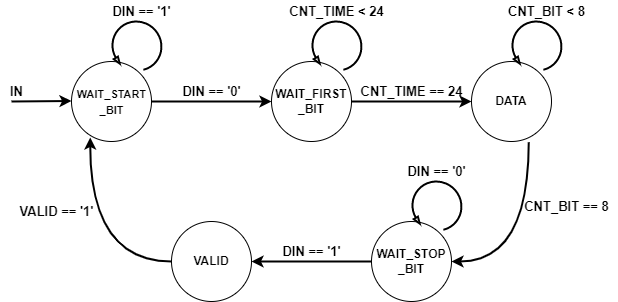
\includegraphics[width=0.85\linewidth]{pic/1ONE.png} 
	\end{center}
	
	
	
	
	
	\subsection{Popis funkce}
	\begin{itemize}
	    \item WAIT\_START\_BIT - čeká na start bit (0)
	    \item WAIT\_FIRST\_BIT - po nalezení start bitu čeká 24 hodinových taktů než začne snímat data (midbit)
	    \item DATA - počet bitu a zápis do registru
	    \item WAIT\_STOP\_BIT - čeká na stop bit (1)
	    \item VALID - nastavení VLD\_DATA na '1' po dobu jednoho taktu
	\end{itemize}
	Celý process spustíme po nastavení start bitu na '0'


%\newpage
%	\section{Snímek obrazovky ze simulaci}
	

\end{document}